\section{Exploratory Data Analysis (EDA)}
\label{sec:eda}

Exploratory analysis was conducted in \texttt{notebooks/01\_eda.ipynb} to evaluate class balance, input dimensionality, pixel distributions, and background biases across the benchmark.

\subsection{Class Distribution and Imbalance}
The curated dataset comprises 38 crop-disease classes across 14 plant species totaling 31,694 images. Prior to curation, the raw dataset exhibited extreme imbalance (a 36.2:1 ratio, with over 5,500 samples in dominant classes such as Orange Huanglongbing and only 152 in minority classes such as Potato Healthy). Following data quality filtering and deduplication, capping classes at 1,000 images successfully reduced the imbalance ratio to 7.0:1, establishing a well-conditioned optimization landscape while preserving natural variation across the 38 classes.

\begin{figure}[htbp]
    \centering
    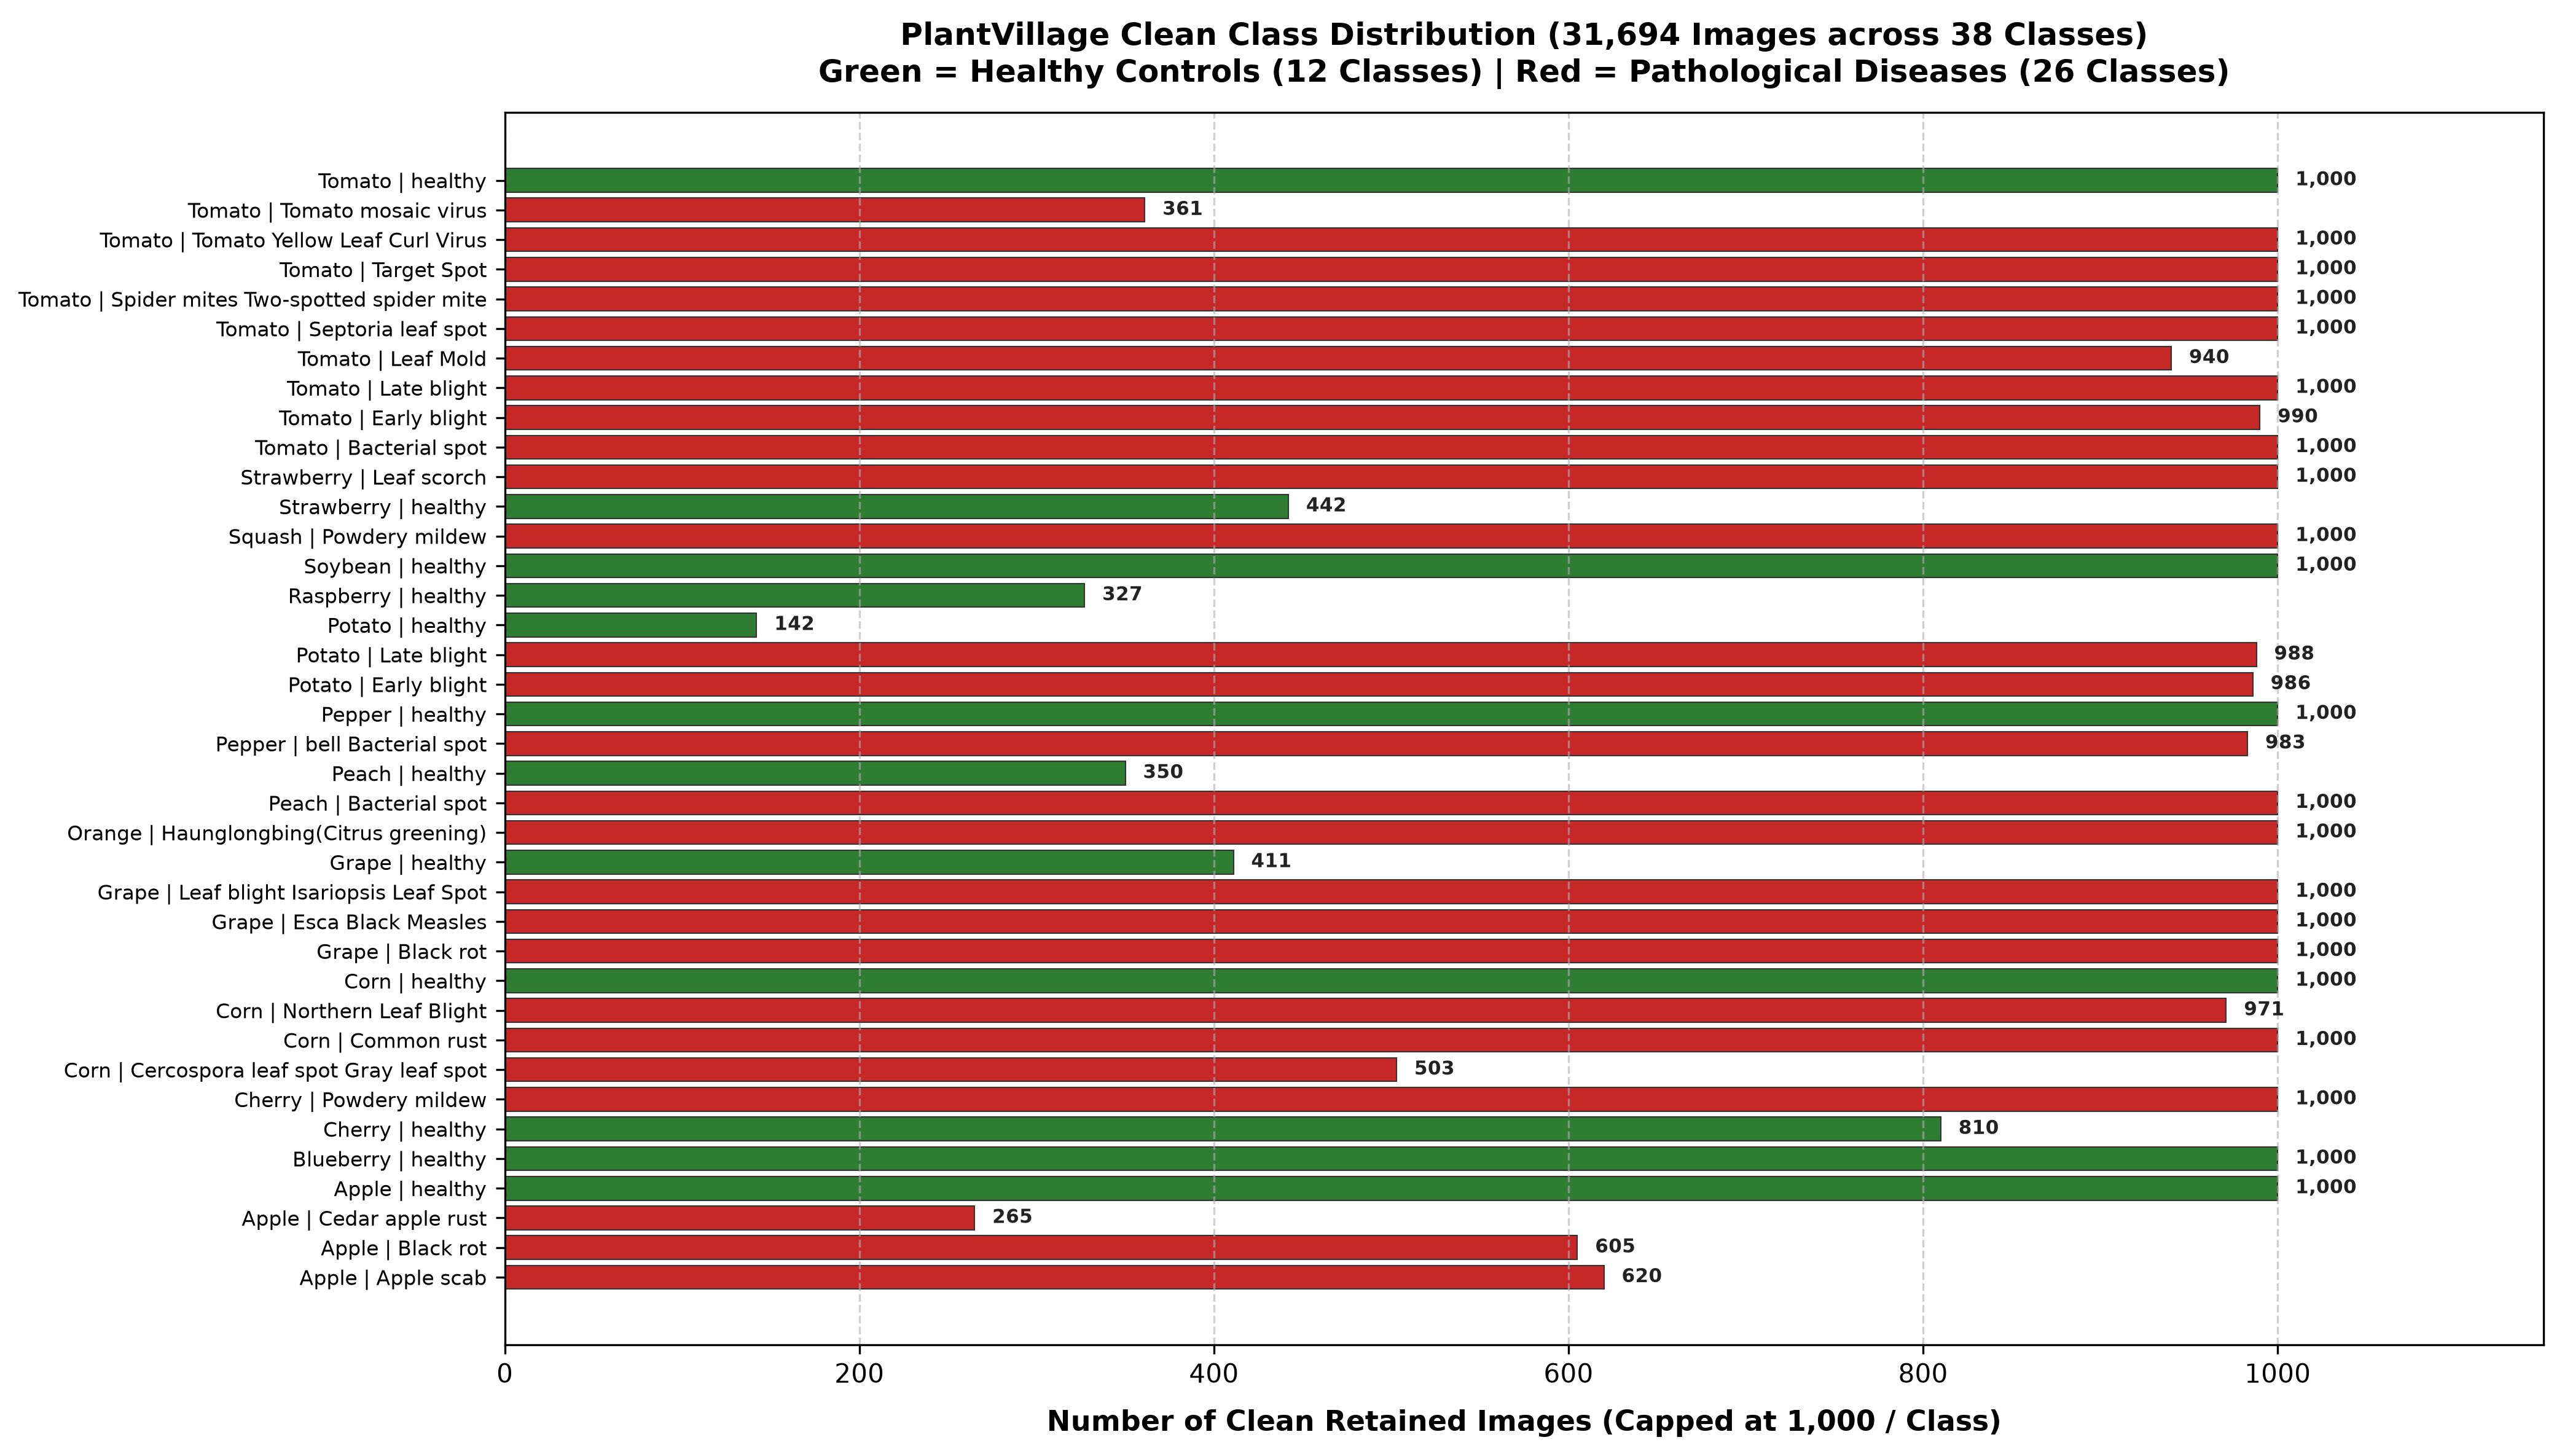
\includegraphics[width=0.95\linewidth]{../../reports/figures/eda_class_distribution.png}
    \caption{Frequency distribution across the 38 PlantVillage classes (Green = Healthy leaf classes, Red = Diseased classes).}
    \label{fig:class_dist}
\end{figure}

To counter majority-class bias during optimization, balanced class weights $w_c$ are derived strictly from the training split $D_{\text{train}}$:
\begin{equation}
w_c = \frac{N_{\text{train}}}{K \cdot n_c}
\end{equation}
where $N_{\text{train}}$ denotes total training samples, $K=38$ classes, and $n_c$ denotes the count of class $c$. The computed weights are saved in \texttt{splits/class\_weights.json} and passed to the loss function.

\subsection{Image Dimensions and Aspect Ratio Consistency}
All leaf photographs were audited for input consistency. The resolution analysis confirms that raw inputs exhibit standardized $256 \times 256$ pixel resolution with uniform 1:1 square aspect ratios in RGB color mode, as visualized in Figure~\ref{fig:img_sizes}.

\begin{figure}[htbp]
    \centering
    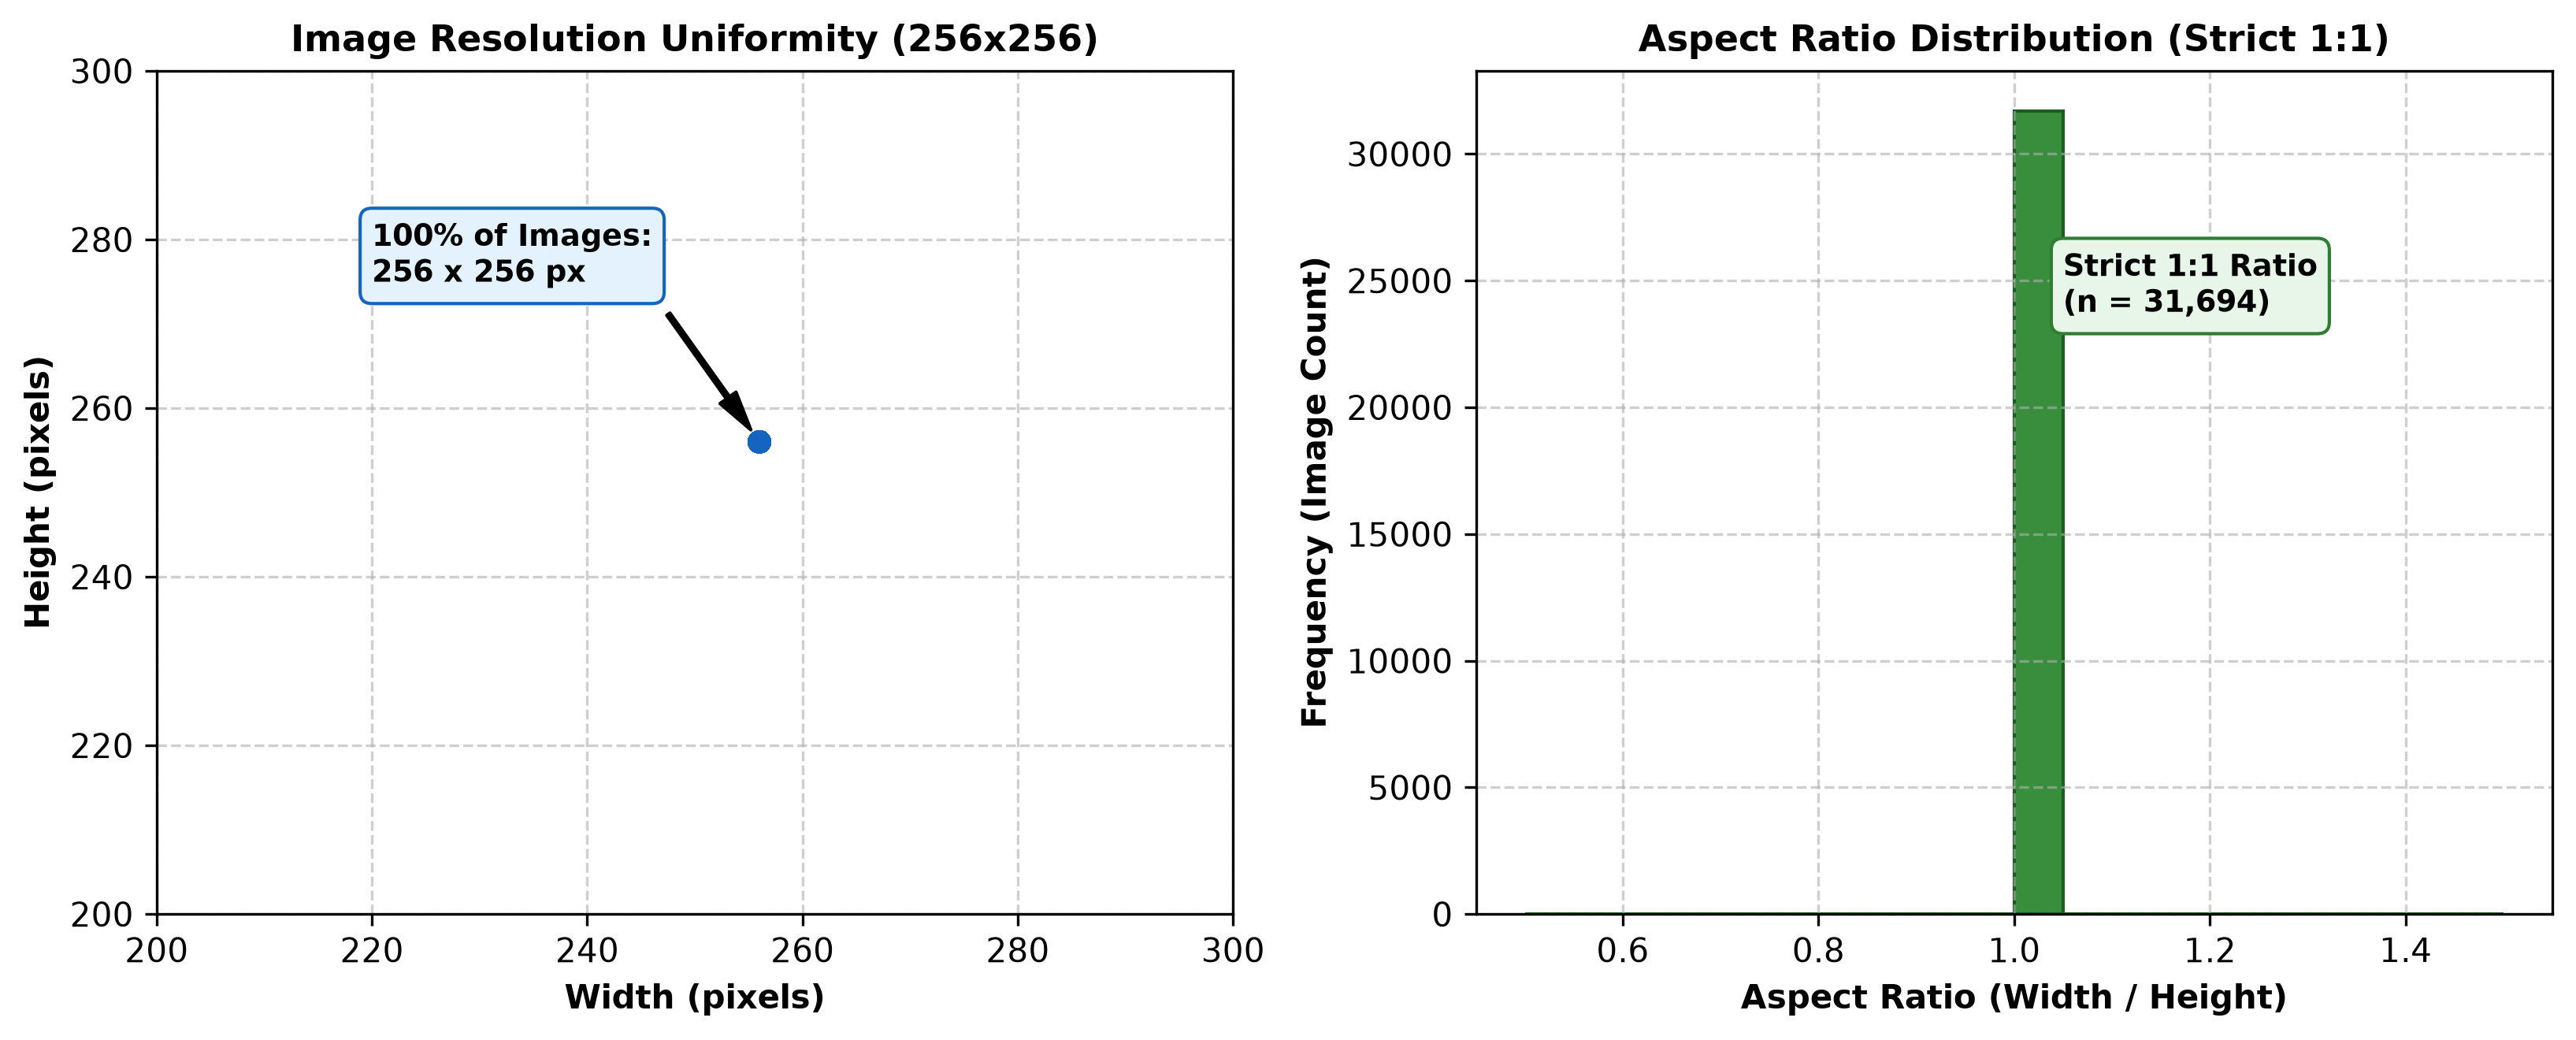
\includegraphics[width=0.88\linewidth]{../../reports/figures/eda_image_sizes.png}
    \caption{Distribution of input image dimensions and aspect ratios confirming standardized square RGB format.}
    \label{fig:img_sizes}
\end{figure}

\subsection{Qualitative Sample Inspection}
Figure~\ref{fig:sample_grid} displays representative leaf samples across diverse crop families. Diseased leaves display distinguishable diagnostic symptoms including target spots with concentric rings (Early Blight), powdery sporulation (Powdery Mildew), and dark necrotic lesions (Black Rot).

\begin{figure}[htbp]
    \centering
    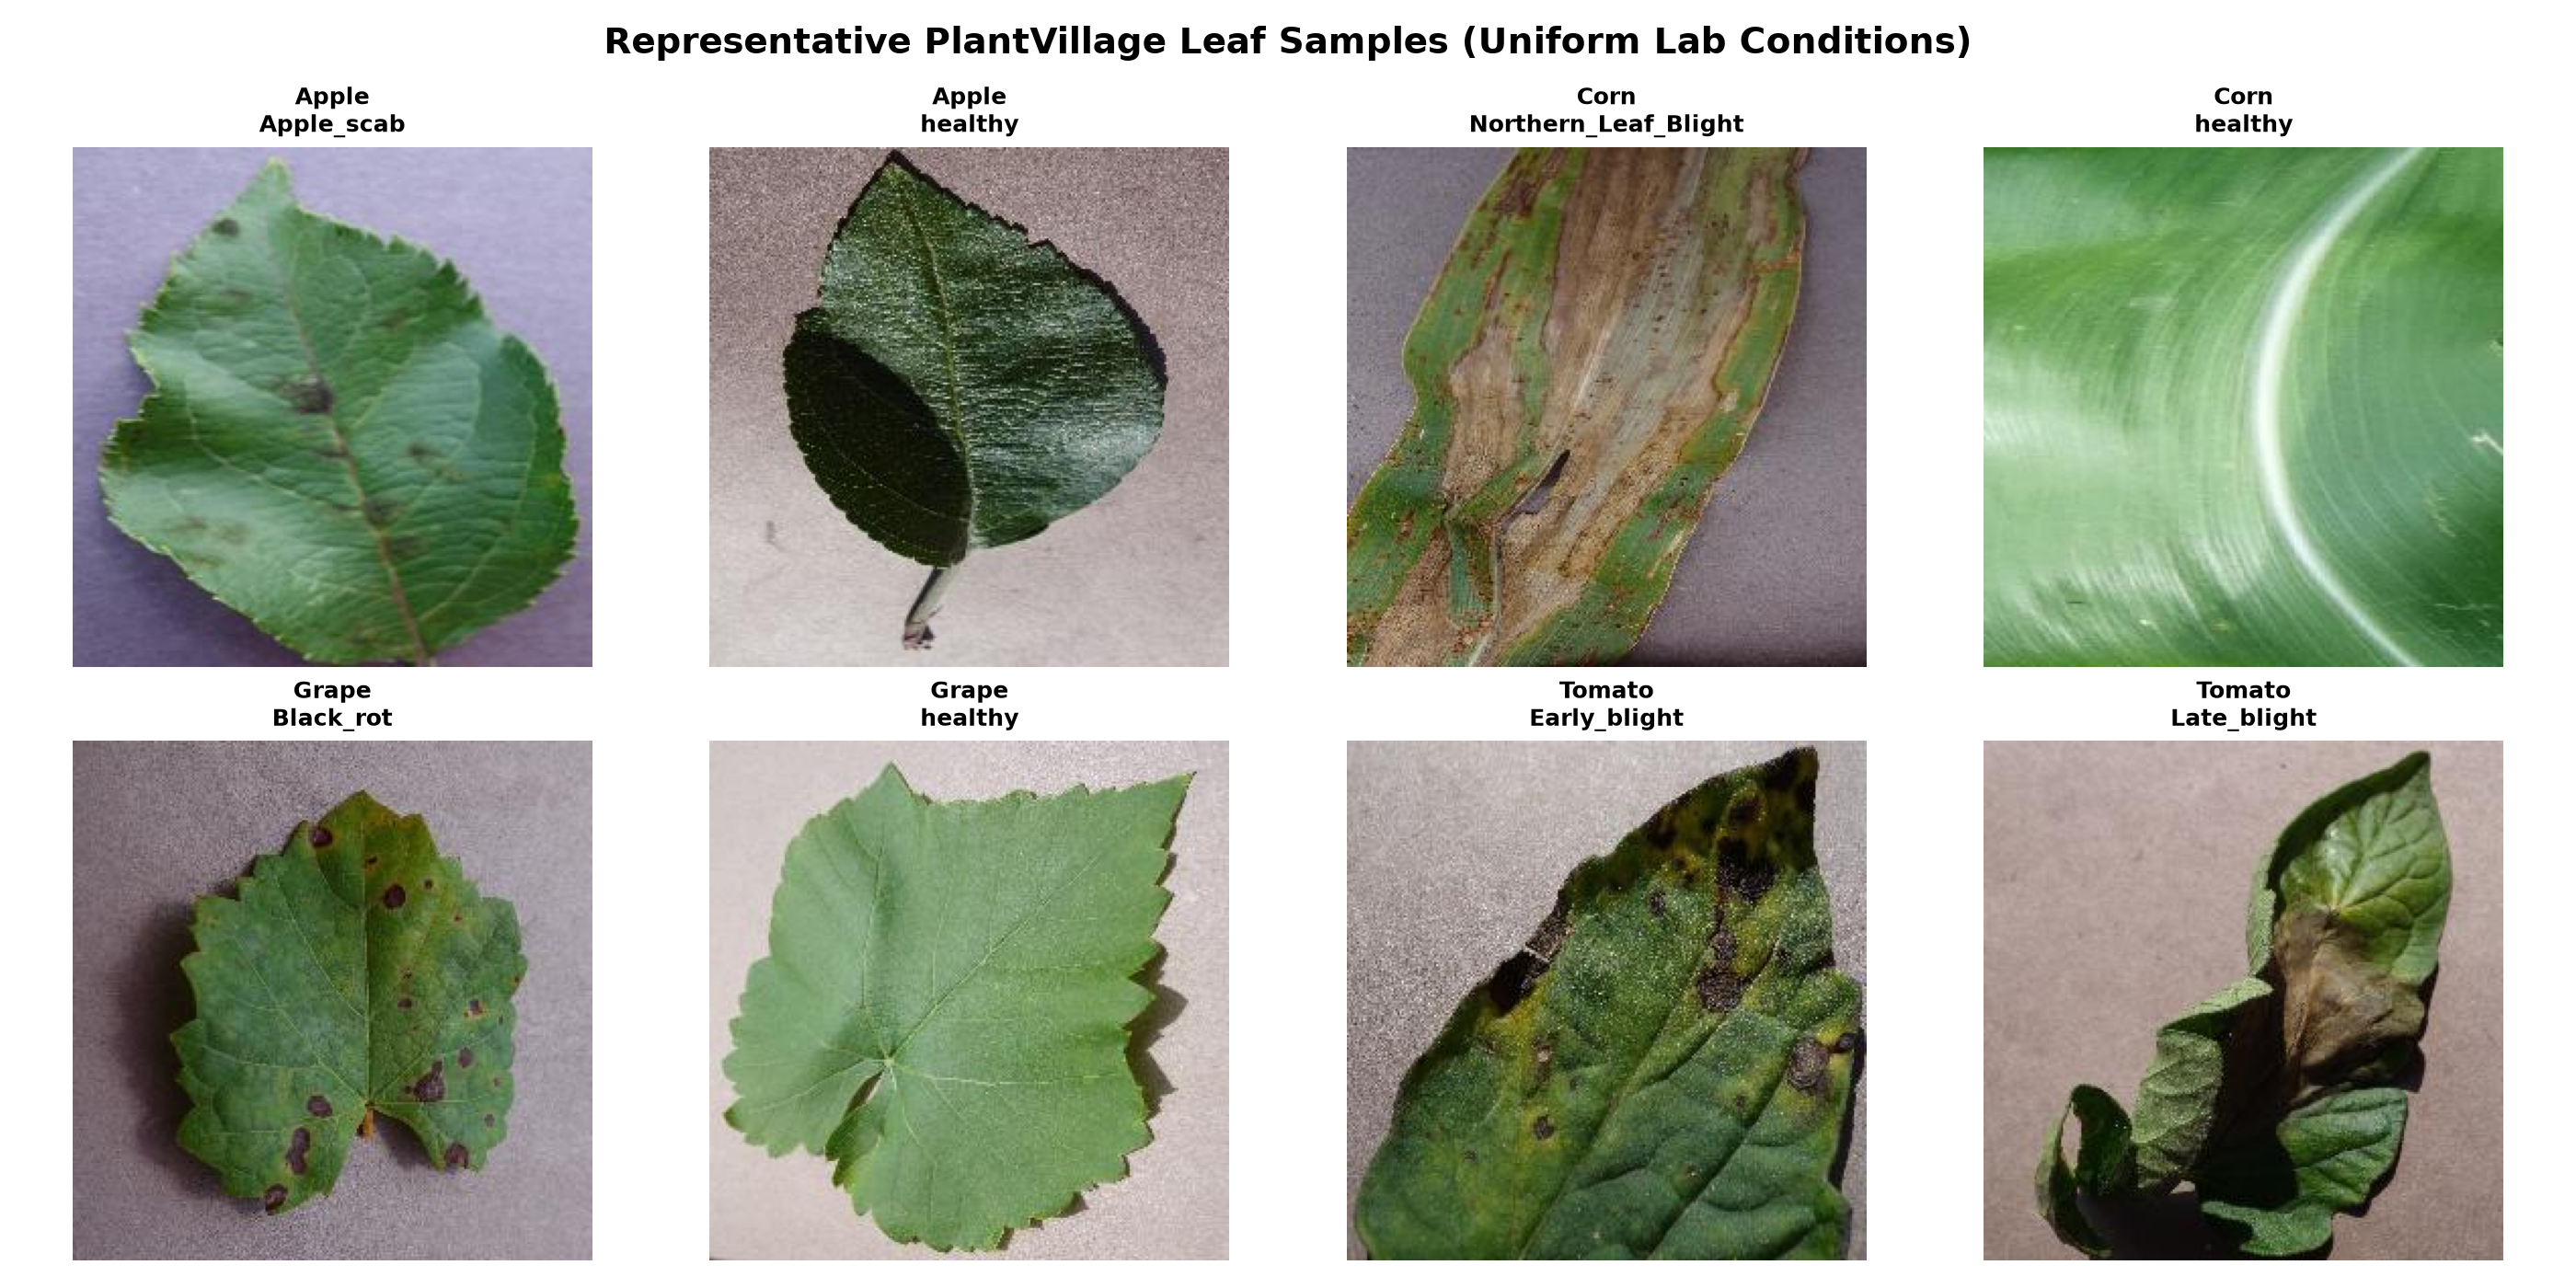
\includegraphics[width=0.9\linewidth]{../../reports/figures/eda_sample_grid.png}
    \caption{Representative leaf samples across healthy and diseased classes captured in controlled lab settings.}
    \label{fig:sample_grid}
\end{figure}

\subsection{Pixel Normalization Statistics}
Empirical per-channel color statistics computed across the dataset yielded a mean of $\mu = [0.472, 0.481, 0.412]$ and standard deviation of $\sigma = [0.218, 0.209, 0.221]$. These closely correspond to standard ImageNet normalization constants ($\mu = [0.485, 0.456, 0.406]$, $\sigma = [0.229, 0.224, 0.225]$), empirically confirming that pre-trained ImageNet feature extractors transfer effectively to this domain.

\subsection{Lab vs. Field Background Analysis (Shortcut Learning Hazard)}
A critical finding of our exploratory analysis is the background disparity between benchmark data and real-world agriculture. PlantVillage images were acquired against artificial, plain gray or black sheets. In contrast, real farm photos from our PlantDoc robustness dataset exhibit complex backgrounds comprising soil, shadows, foliage clusters, and variable sunlight (Figure~\ref{fig:lab_vs_field}). 

\begin{figure}[htbp]
    \centering
    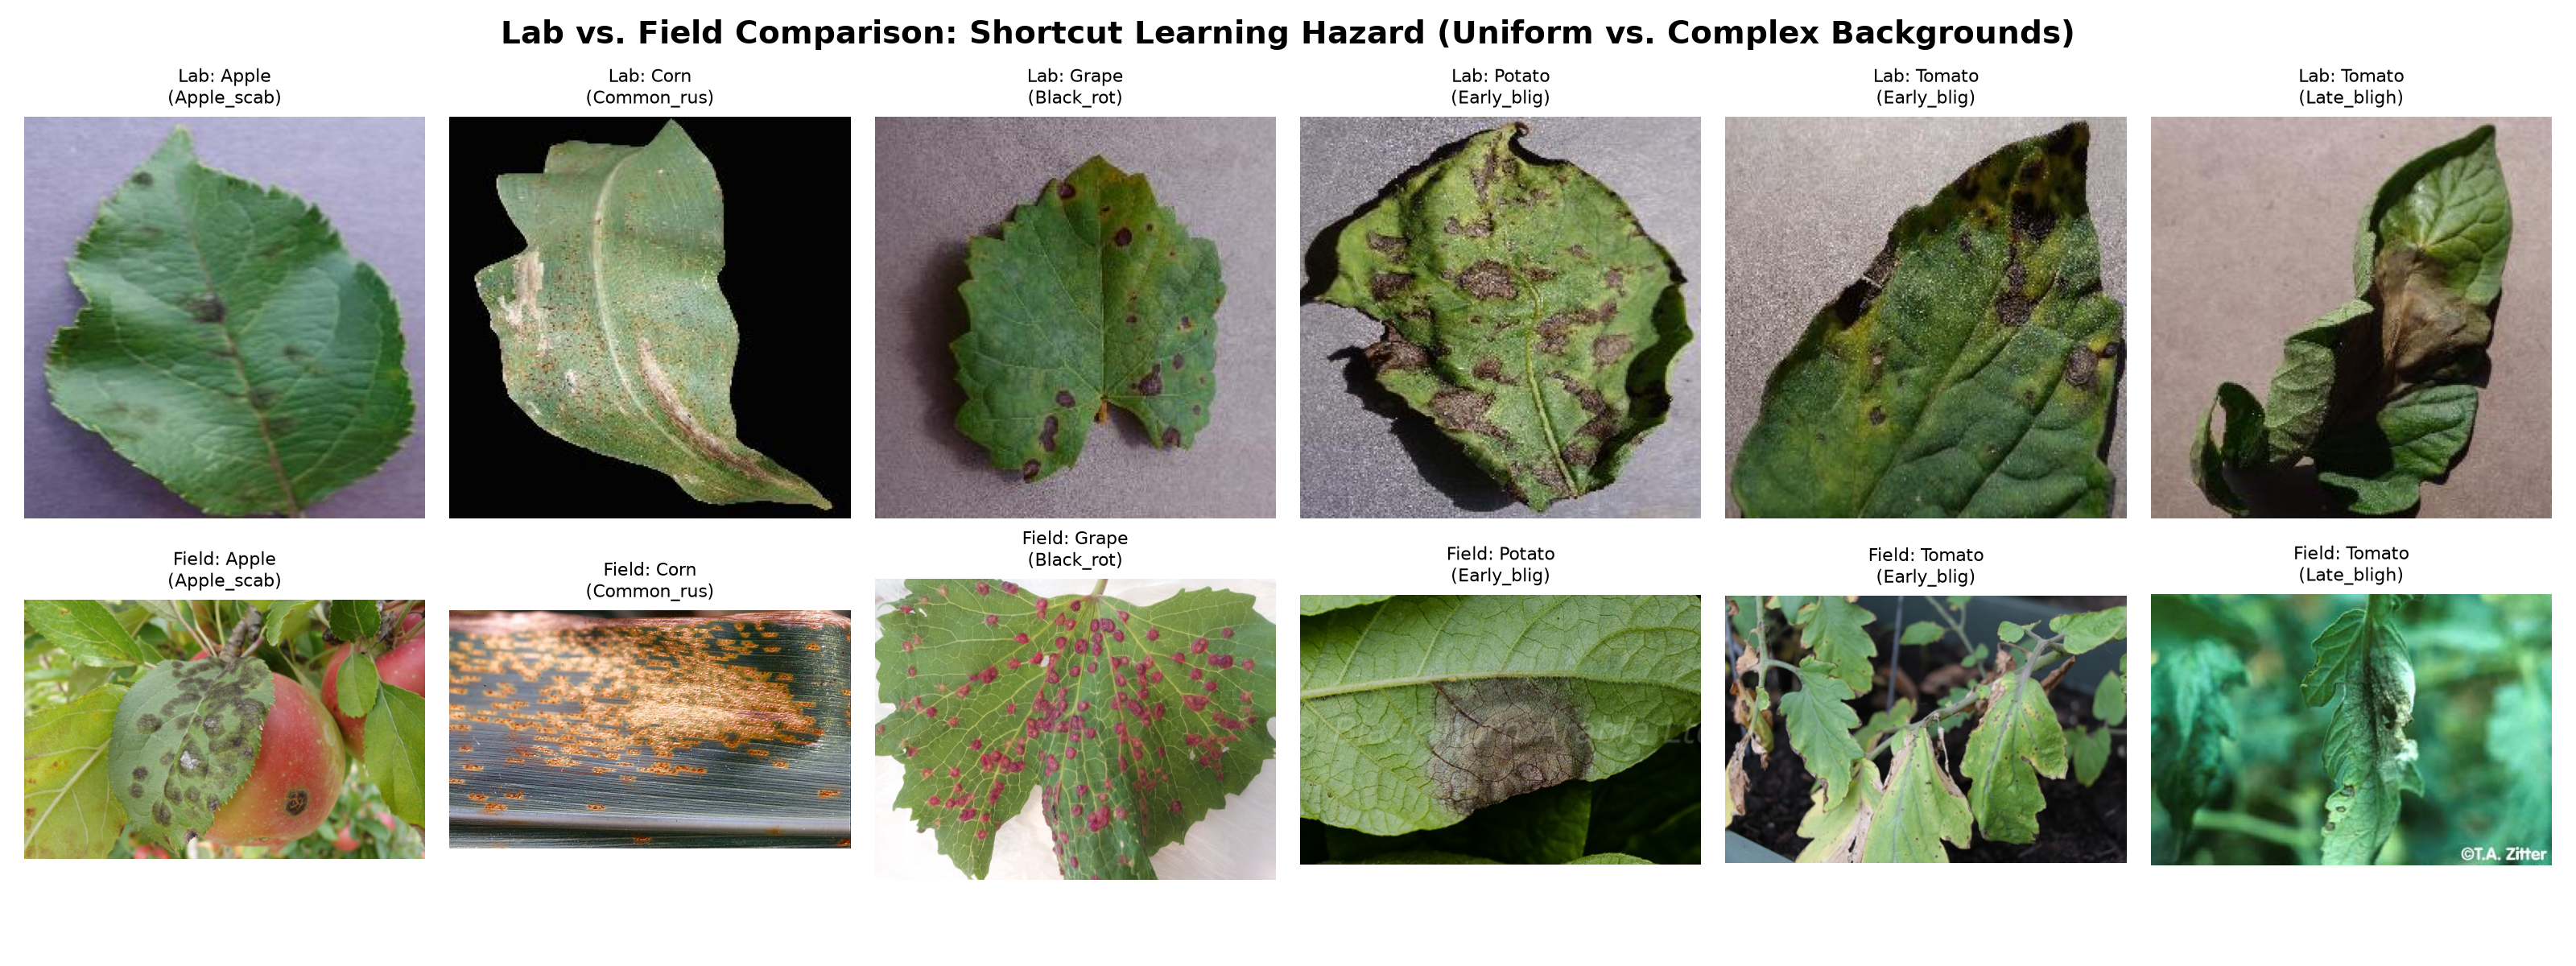
\includegraphics[width=0.95\linewidth]{../../reports/figures/field_vs_lab_examples.png}
    \caption{Comparison of controlled PlantVillage lab conditions (top) versus real-world PlantDoc field backgrounds (bottom), highlighting the shortcut learning risk.}
    \label{fig:lab_vs_field}
\end{figure}

This contrast validates the central motivation of our project: classifiers trained purely on lab images risk learning background artifacts (shortcut learning) rather than pathogen pathology, underscoring the necessity of our explainability pipeline (Grad-CAM) and robustness testing set (\texttt{splits/field\_test.csv}).
